\appendix

\sect{Tree Structure}

\subsect{Flattening}

A tree can be flattened for root-first traversal based on either breadth-first
search (BFS) or depth first search (DFS).

\begin{itemize}
	\item $i$ is the zero-indexed traversal order, corresponding to an array
	index of the flattened tree.
	\item $m$ is the branching factor of the tree.
	\item $h$ is the height of the tree.
	\item $r$ is the ``row'' where a given node resides in the tree;
	the number of tree levels removed from the root.
	\item $c$ is the ``column'' where a given node resides  in the tree;
	the number of nodes away from the left edge.
\end{itemize}


\begin{figure}[H]
	\centering
	\begin{tikzpicture}[
			xscale=0.7,
			tree/.style={draw,circle,inner sep=0.25mm, minimum size=14pt}
		]
		\node[tree] at (0, 0) (00) {$0,0$};
		\foreach \r [
			evaluate = \r as \w using int(3^\r),
			evaluate = \r as \wl using int(3^\r-1)
		] in {1,...,2} {
			% Columns
			\foreach \c [
				evaluate = \c as \i using int((\w-1)/2 + \c),
				evaluate = \c as \pr using int(\r-1),
				evaluate = \c as \pc using int(\c/3),
			] in {0,...,\wl} {
				\node[tree] (\r\c)
					at (\c, -\r) {$\r,\c$};
				\draw[-] (\pr\pc.south)
					-- ++(0, {-((3-\pc) + (\pr-1))/9}) -| (\r\c);
			}
		}
		\node[anchor=east] (legend) at (00 -| 28) {Node text is $r,c$};
		\node[anchor=east, below=0.1 of legend] {$m=3, h=3$};
	\end{tikzpicture}
\end{figure}


\subsubsect{BFS}

$$
	i = c + \sum_{k=1}^r m^k
	= c + \frac{1 - m^r}{1 - m}
$$

\tikzmath{\treem = 3; \treeh = 3;}

\begin{figure}[H]
	\centering
	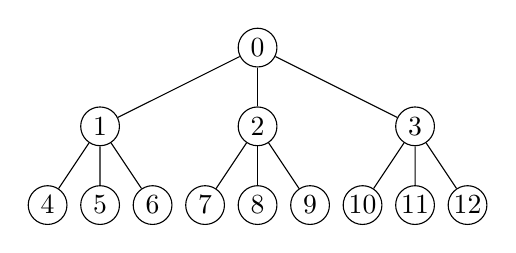
\begin{tikzpicture}[
			xscale=1.2,
			tree/.style={draw,circle,inner sep=0.25mm, minimum size=14pt}
		]
		\node[tree] at (0, 0) (00) {0};
		\foreach \r [
			evaluate = \r as \w using int(3^\r),
			evaluate = \r as \wl using int(3^\r-1)
		] in {1,...,2} {
			% Columns
			\foreach \c [
				evaluate = \c as \i using int((\w-1)/2 + \c),
				evaluate = \c as \pr using int(\r-1),
				evaluate = \c as \pc using int(\c/3),
			] in {0,...,\wl} {
				\node[tree] (\r\c)
					at ({(\c-int(\w/2)) / (\w/5)}, -\r) {\i};
				\draw[-] (\pr\pc) -- (\r\c);
			}
		}
	\end{tikzpicture}
\end{figure}


\subsubsect{DFS}

$$
	i = r + c\sum_{k=1}^{h-r} m^k
		+ \sum_{k=1}^{h-2} \left\lfloor\frac{c}{m^k}\right\rfloor
	= r + c\pfrac{1 - m^{h-r}}{1 - m}
		+ \sum_{k=1}^{h-2} \left\lfloor\frac{c}{m^k}\right\rfloor
$$

\begin{figure}[H]
	\centering
	\begin{tikzpicture}[
			xscale=1.2,
			tree/.style={draw,circle,inner sep=0.25mm, minimum size=14pt}
		]
		\node[tree] at (0, 0) (00) {0};
		\foreach \r [
			evaluate = \r as \w using int(3^\r),
			evaluate = \r as \wl using int(3^\r-1)
		] in {1,...,2} {
			% Columns
			\foreach \c [
				evaluate = \c as \i using int(
					\r + \c*(
						1 - (\treem^(\treeh-\r))
					)/(
						1 - \treem
					) + int(\c/3) + int(\c/9)
				),
				evaluate = \c as \pr using int(\r-1),
				evaluate = \c as \pc using int(\c/3),
			] in {0,...,\wl} {
				\node[tree] (\r\c)
					at ({(\c-int(\w/2)) / (\w/5)}, -\r) {\i};
				\draw[-] (\pr\pc) -- (\r\c);
			}
		}
	\end{tikzpicture}
\end{figure}


\subsect{Choosing Tree Parameters}

A level $k$ down the tree from the root will contain $m^k$ nodes.
Thus, a tree of with $h$ levels will contain
$\sum_{k=1}^h m^k = \frac{1-m^h}{1-m}$ nodes.

The ratio of leaf nodes to internal nodes is given by:
$$
	\frac{m^{h-1}}{\pfrac{1-m^{h-1}}{1-m}}
	= \frac{m^{h-1}(1-m)}{1-m^{h-1}}
	= \frac{m^{h-1}-m^{h}}{1-m^{h-1}}
	% = \frac{m^h-m^{h+1}}{m-m^h}
	% = \frac{m^h(1-m)}{m^h(m^{1-h} - 1)}
	= \frac{1-m}{m^{1-h} - 1}
$$

As $h$ increases, this rapidly converges to $m$.

\begin{figure}[H]
	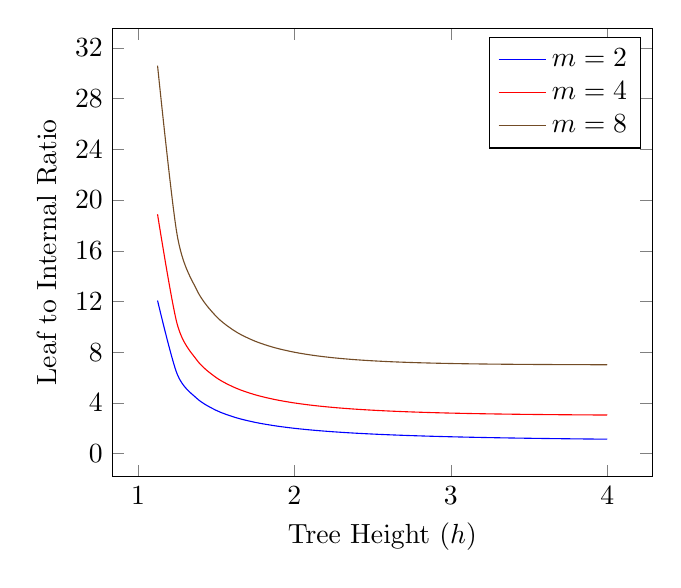
\begin{tikzpicture}
		\begin{axis}
			[
				xlabel={Tree Height ($h$)},
				ylabel={Leaf to Internal Ratio},
				xtick distance=1,
				ytick distance=4,
				domain=1:4,
				smooth
			]
			\pgfplotsinvokeforeach{2,4,8} {
				\addplot+[cycle list name=auto, mark=none]
					{(1-#1) / (#1^(1-x) - 1)};
				\addlegendentry{$m=#1$}
			}
		\end{axis}
	\end{tikzpicture}
\end{figure}

As the height of a tree grows, the portion of overall memory that is used for
leaves decreases, converging to $1-\frac{1}{m}$. Higher branching factors spend
less memory on traversal data. Recall that internal nodes do not store data;
they store pointers to other nodes to accelerate lookups over a flat ordered
list. Such a flat list of $n$ elements is equivalent to a B-Link tree of $m=n$
and $h=1$.

\begin{figure}[H]
	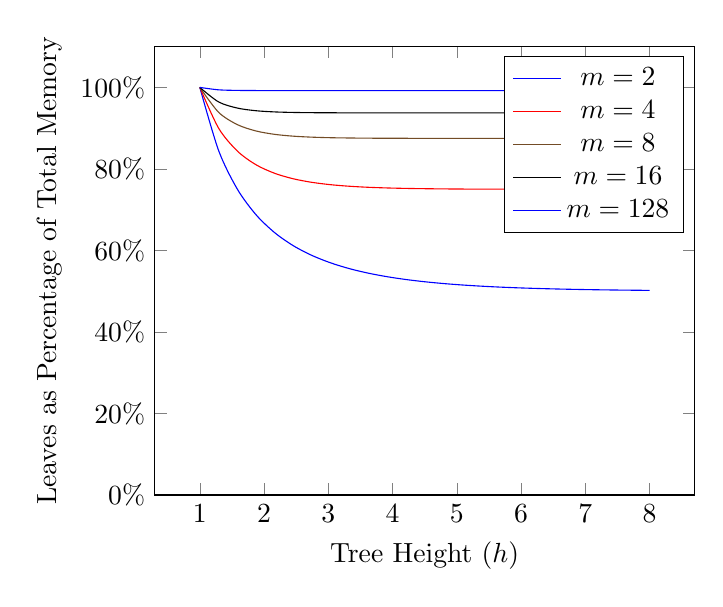
\begin{tikzpicture}
		\begin{axis}
			[
				xlabel={Tree Height ($h$)},
				ylabel={Leaves as Percentage of Total Memory},
				xtick distance=1,
				yticklabel={%
					\pgfmathparse{\tick*100}%
					\pgfmathprintnumber{\pgfmathresult}%
					\%%
				},
				domain=1:8,
				ymin=0,
				smooth
			]
			\pgfplotsinvokeforeach{2,4,8,16,128} {
				\addplot+[cycle list name=auto, mark=none]
					{#1^(x-1) / ((1-#1^x)/(1-#1))};
				\addlegendentry{$m=#1$}
			}
		\end{axis}
	\end{tikzpicture}
\end{figure}

A tree containing $N$ nodes will have the height shown below.

\begin{align*}
	N &= \frac{1-m^h}{1-m} \\
	N (1-m) &= 1-m^h \\
	N (1-m) - 1 &= -m^h \\
	1 - N (1-m) &= m^h \\
	\log_m\left(1 - N (1-m)\right) &= h
\end{align*}

\begin{figure}[H]
	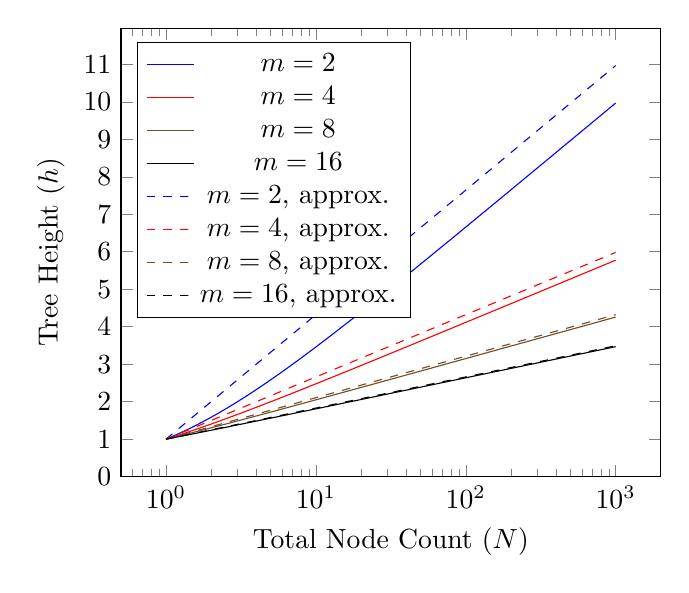
\begin{tikzpicture}
		\begin{axis}
			[
				xlabel={Total Node Count ($N$)},
				ylabel={Tree Height ($h$)},
				domain=1:1000,
				xmode=log,
				ytick distance=1,
				legend pos=north west,
				smooth
			]
			\pgfplotsinvokeforeach{2,4,8,16} {
				\addplot+[cycle list name=auto, mark=none]
					{ln(1 - x*(1-#1)) / ln(#1)};
				\addlegendentry{$m=#1$}
			}
			\pgfplotsinvokeforeach{2,4,8,16} {
				\addplot+[cycle list name=auto, mark=none, dashed]
					{1+ln(x)/ln(#1)};
				\addlegendentry{$m=#1$, approx.}
			}
		\end{axis}
	\end{tikzpicture}
\end{figure}

As $N$ grows, this relation can be approximtaed as $h = 1 + \frac{\log N}{\log m}$

\begin{figure}[H]
	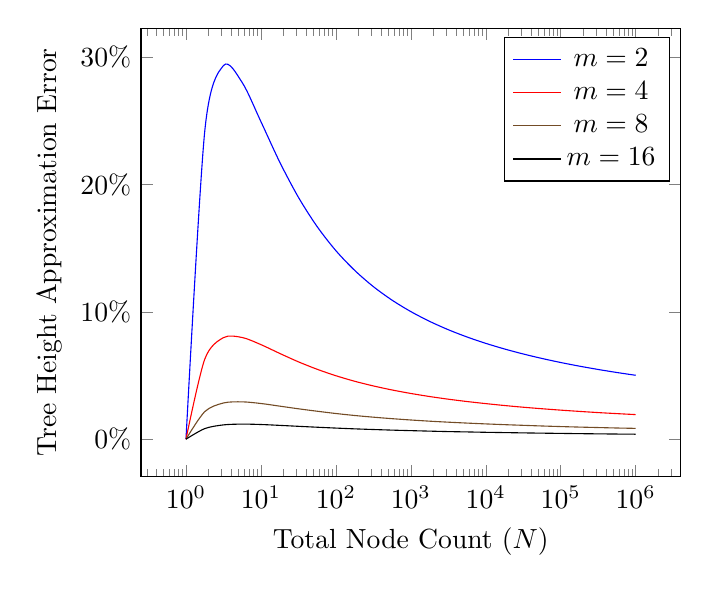
\begin{tikzpicture}
		\begin{axis}
			[
				xlabel={Total Node Count ($N$)},
				ylabel={Tree Height Approximation Error},
				domain=1:1000000,
				xmode=log,
				yticklabel={%
					\pgfmathparse{\tick*100}%
					\pgfmathprintnumber{\pgfmathresult}%
					\%%
				},
				smooth
			]
			\pgfplotsinvokeforeach{2,4,8,16} {
				\addplot+[cycle list name=auto, mark=none]
					{
						(
							(
								1+ln(x)/ln(#1)
							) - (
								ln(1 - x*(1-#1)) / ln(#1)
							)
						) / (
							ln(1 - x*(1-#1)) / ln(#1)
						)
					};
				\addlegendentry{$m=#1$}
			}
		\end{axis}
	\end{tikzpicture}
\end{figure}
